% ---------
%  Compile with "pdflatex hw0".  
% --------
%!TEX TS-program = pdflatex

\documentclass[11pt]{article}
\usepackage{jeffe,handout,graphicx}

% ---------
% Input file uses Unicode's UTF-8 encoding
% ---------
%!TEX encoding = UTF-8 Unicode
\usepackage[utf8]{inputenc}

% ---------
%  The next several lines (up to the line of =='s) change the default text
%  and math fonts and make a few other minor cosmetic changes.  If you get
%  any error messages related to these packages, just comment them out.
%         -- Jeff
% --------
\usepackage[charter]{mathdesign}
\def\sfdefault{fvs}
\def\ttdefault{fvm}
\SetMathAlphabet{\mathsf}{bold}{\encodingdefault}{\sfdefault}{b}{\updefault}
\SetMathAlphabet{\mathtt}{bold}{\encodingdefault}{\ttdefault}{b}{\updefault}
\SetMathAlphabet{\mathsf}{normal}{\encodingdefault}{\sfdefault}{\mddefault}{\updefault}
\SetMathAlphabet{\mathtt}{normal}{\encodingdefault}{\ttdefault}{\mddefault}{\updefault}
\usepackage{microtype}
% ---------
%  End of cosmetics.
% --------

% ---------
%  Redefine suits
% --------
\usepackage{pifont}
\def\Spade{\ding{171}}
\def\Heart{\textcolor{Red}{\ding{170}}}
\def\Diamond{\textcolor{Red}{\ding{169}}}
\def\Club{\ding{168}}


\newtheorem{lemma}{Lemma}

% =========================================================
\begin{document}

\headers{CS 573 HW0}{}{Alina Ene (ene1), Jeff Erickson (jeffe), Aloisius P. Hassenpfeffer (aphassen)}

\small\sf	% typeset excetps from problems in a different, smaller font

\begin{enumerate}
\item
\begin{enumerate}\itemsep 2ex plus 0.1fil
\item[(•)]
\textcolor{red}{\EMPH{Write the sentence ``I understand the course policies."}}

\begin{solution}
\textcolor{red}{\textbf{I turned this in without reading it.}}
\end{solution}

\item
Solve the recurrences.

\begin{solution}
\begin{align*}
	A(n) &= \Theta(\pi^n) \\
	B(n) &= \Theta(\sqrt{\log^* n}) \\
	C(n) &= \Theta(1/n) \\
	D(n) &= \Theta(42) \\
	E(n) &= \Theta(2^{e\ln n \ln \ln n}/\alpha(n)) \\
\end{align*}
\end{solution}

\item
Sort the functions from asymptotically smallest to asymptotically largest, indicating ties if any.

\begin{solution}
\begin{align*}
		n
	& \ll
		\varnothing  & \text{[the empty set]} \\
	& \ne
		\phi  & \text{[the golden ratio $(1+\sqrt{5})/2$]}\\
	& \equiv
		\text{bacon} \\
	& \subseteq 
		\text{chunky bacon} \\
	& \ge
		\sqrt{n} \\
	& \lhd
		\set{4, 8, 15, 16, 23, 42, \text{hike!}} \\
	& \not\sqsubseteq
		7\cdot\sqrt{7^n} \\
	& \Join
		7^{\lg n^7}\lg n \\
	& \cong
		\lg( 7^{7^{\cdots^7}}) \\
	& \models
		(7!)^{\lg \sqrt{n!}}! \\
	& \doteqdot
		\sqrt{7777777^{\sqrt{7777777}}} \\
	& \Bumpeq
		\frac{\sqrt[7]{7^{\sin n}}}{7} \\
	& \succeq
		\lg\lg\lg\lg (7^{\sqrt{\beta(\text{acon})}}) \\
	& \ncong
		\log^* \sqrt{7^n} \\
	& \ddot{\smallsmile}
		\sqrt{\lg \left(7^{\sqrt{\lg (7^n)}}\right)}
	\end{align*}
\end{solution}

\end{enumerate}

%----------------------------------------------------------------------
\def\symbol#1{\textbf{\texttt{#1}}}
\newpage
\item
\begin{enumerate}
\item
List the nodes in Prof. della Giungla's tree in the order visited by a \emph{preorder} traversal. 

\begin{solution}
\symbol{M Y B O L O G N A H A S A F I R S T N A M E I T S O S C A R}
\end{solution}

\item
Draw Prof. della Giungla's tree.

\begin{solution}~

\begin{center}
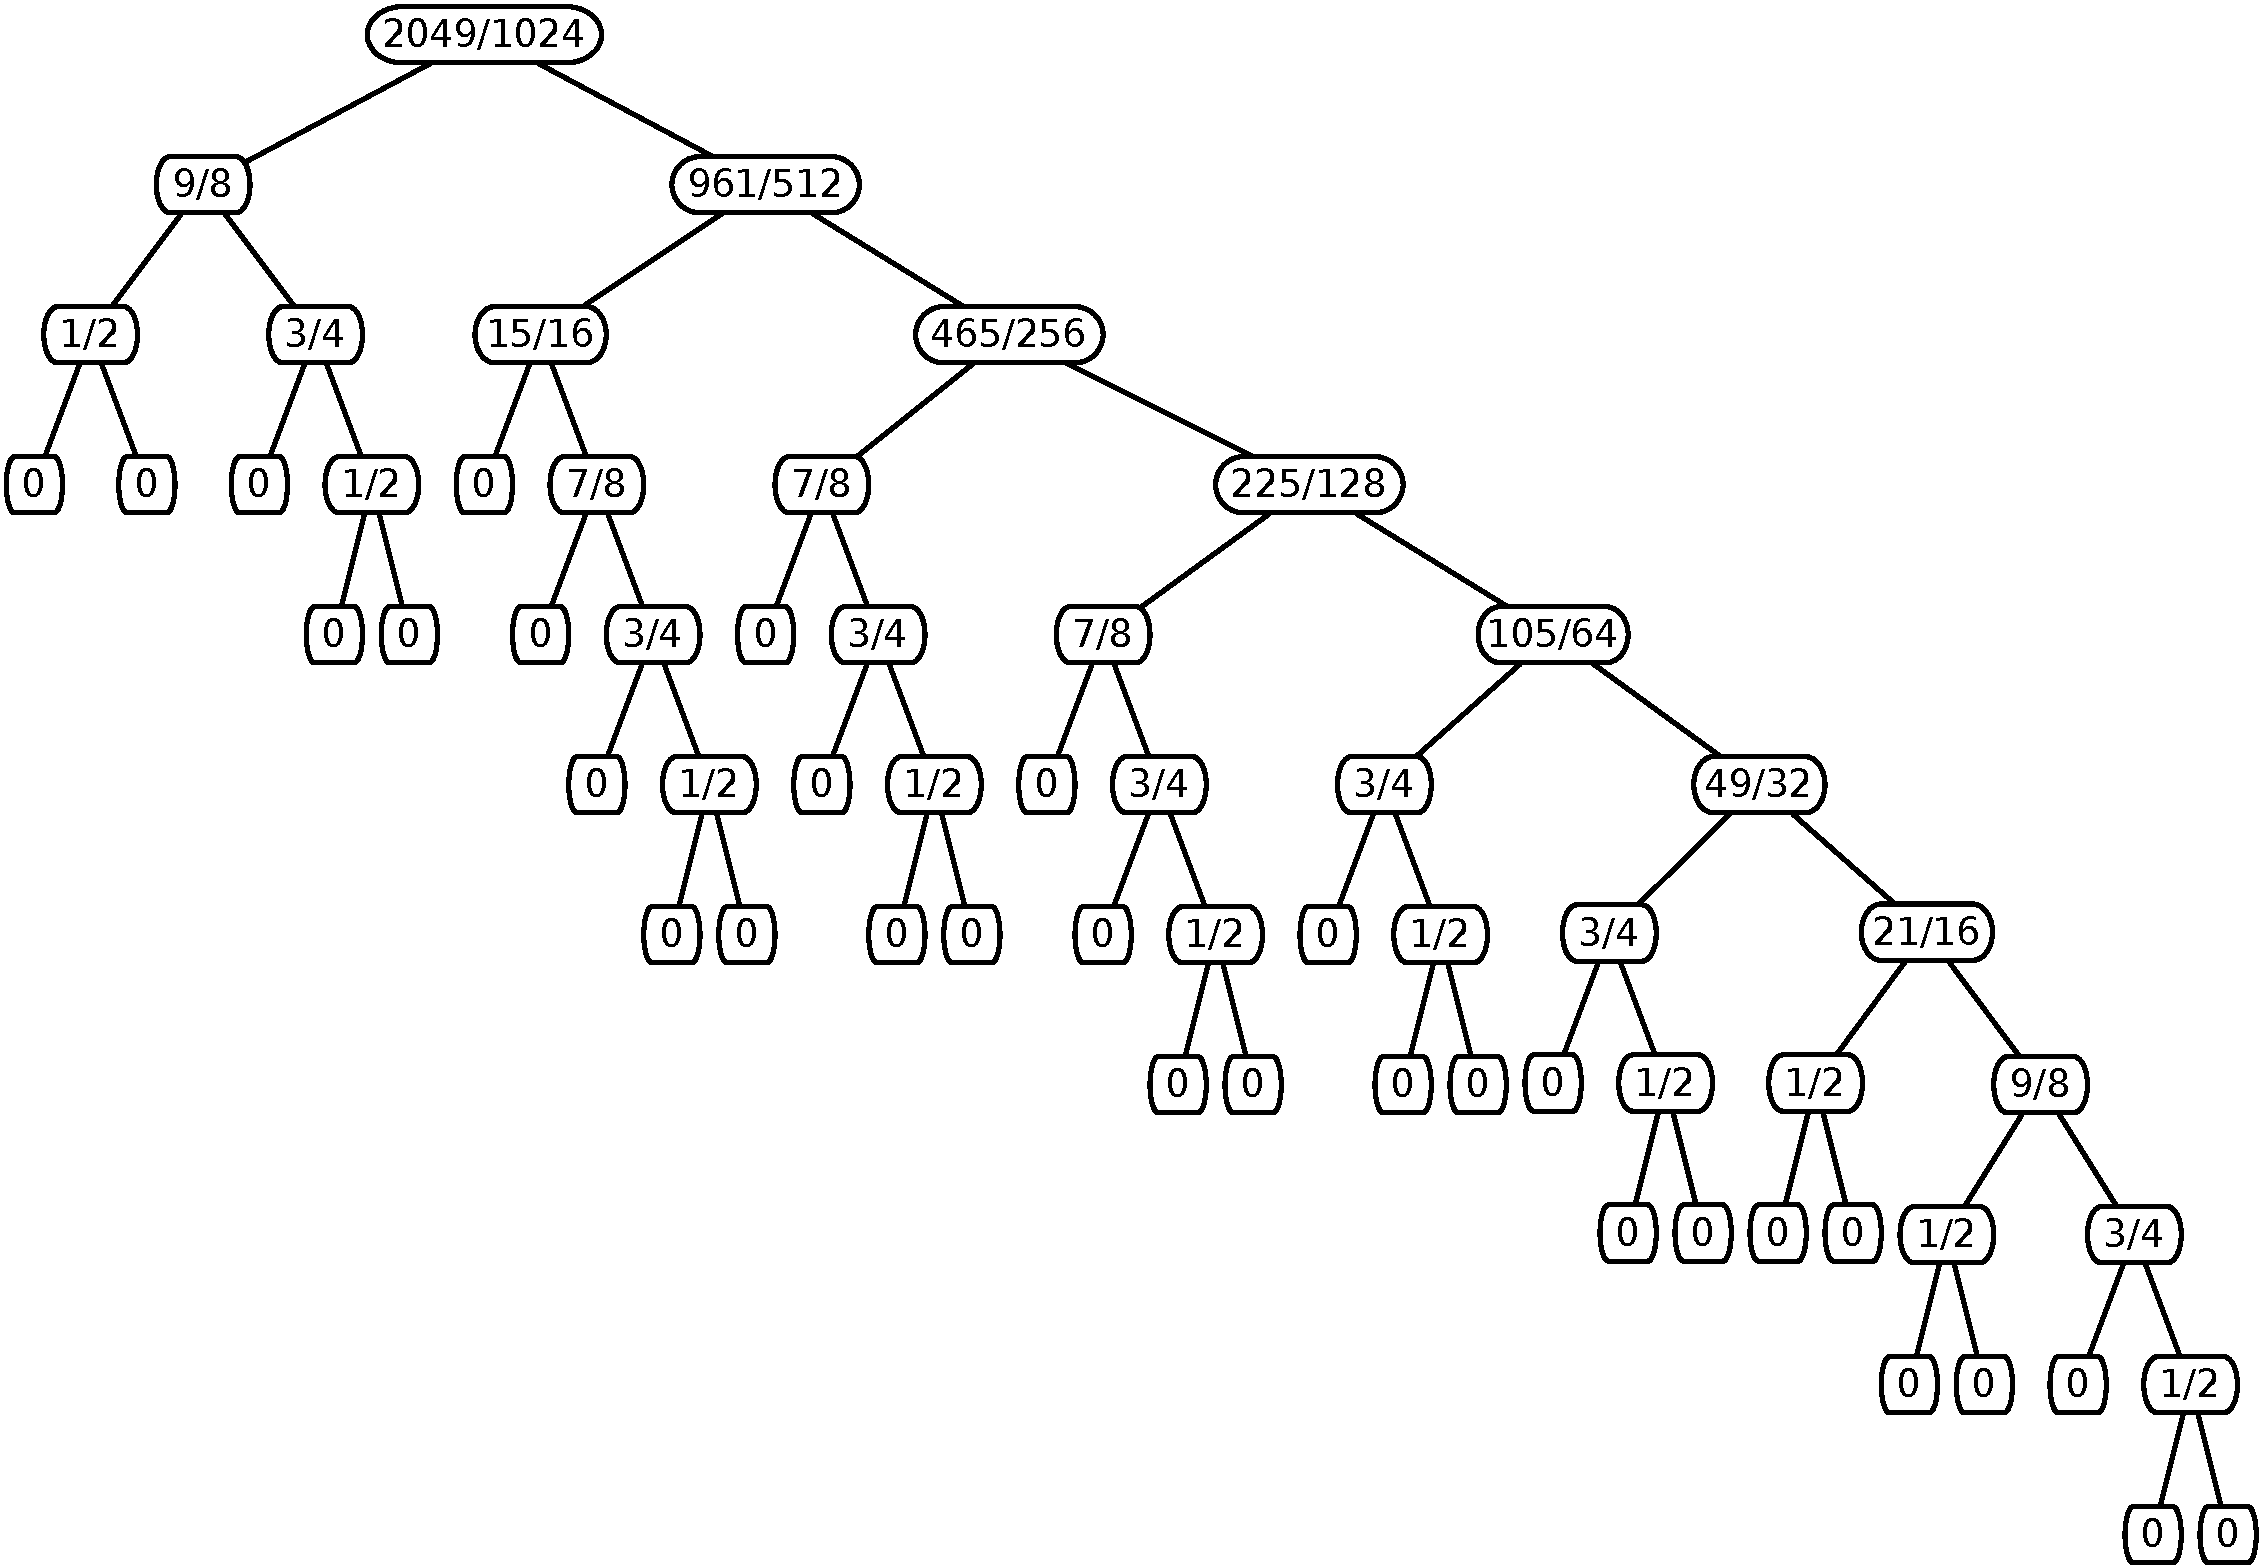
\includegraphics[height=3.5in]{Fig/wrong-tree}
\end{center}
\end{solution}

\end{enumerate}

%----------------------------------------------------------------------
\newpage
\item
Describe a data structure that stores a set of $n$ points in the plane and supports the queries \textsc{\textrm{LowestToRight}} and \textsc{\textrm{LeftmostAbove}}.

\begin{solution}
Alles touristen und non-technischen looken peepers! Das machinkontrol is nicht for gefengerpoken und mittengrabben. Oderwise is easy schnappen der springenverk, blowenfus, undpoppencorken mit spitzensparken. Der machine is diggen by experten only. Is nicht fur geverken by das dumpkopfen. Das rubber necken sightseenen keepen das cotton-picken hands in das pockets. So relaxen, und vatchen das blinkenlights. 

\begin{center}\small
\begin{algorithm}
\textul{$\mathsc{PeasantMultiply}(x,y)$:}\+
\\	$\emph{prod}\gets 0$
\\	while $x > 0$\+
\\		if $x$ is odd\+
\\			$\emph{prod} \gets \emph{prod} +y$\-
\\		$x \gets \floor{x/2}$
\\		$y \gets y+y$\-
\\	return $p$
\end{algorithm}
\end{center}

\emph{This room is fullfilled mit special electronische equipment. Fingergrabbing and pressing the knoeppkes from the computers is allowed for die experts only! So all the "lefthanders" stay away and do not disturben the brainstorming von here working intelligences. Otherwise you will be outthrown and kicked anderswhere! Also: please keep still and only watchen astaunished the blinkenlights. }
\end{solution}

%----------------------------------------------------------------------
\newpage
\item
Prove that for any arithmetic expression tree, there is an equivalent arithmetic expression tree in normal form.


\begin{solution}
Lorem ipsum dolor sit amet, consectetur adipiscing elit. Nunc molestie blandit feugiat. Donec vitae mi in risus aliquam posuere sed quis arcu. Vestibulum orci nibh, commodo sit amet pulvinar sed, porttitor in justo. Quisque nec est ipsum, non pretium velit. Vestibulum pulvinar vestibulum justo, quis molestie felis aliquam sed. Vivamus dapibus posuere ipsum eget vehicula. Mauris id fringilla leo. Aenean id mauris arcu, egestas tristique nisl. Proin sed dui a felis porttitor blandit eu sit amet quam. Cras vel dolor magna. Cras sit amet elit turpis, quis convallis dui. Suspendisse vestibulum, massa in aliquam rutrum, nunc metus fermentum tortor, at feugiat eros odio ac turpis. Curabitur ligula odio, elementum vel laoreet in, pulvinar id urna.

\begin{lemma}
Suspendisse suscipit ullamcorper bibendum. Cras tellus leo, interdum sit amet commodo sit amet, fermentum vel diam.
\end{lemma}

\begin{proof}
Cras ut tristique massa. Maecenas in nulla est. Nullam vel leo nec est viverra viverra. Donec dapibus, lorem vitae vestibulum interdum, leo nulla blandit magna, laoreet congue nibh lorem nec quam. Class aptent taciti sociosqu ad litora torquent per conubia nostra, per inceptos himenaeos. Fusce tristique dui in leo vestibulum ultricies. Nam dictum neque at arcu placerat vehicula. Aenean lectus leo, rutrum eget dignissim sit amet, mattis nec lorem.
\[
	S(e^d) := \sum_{con=sec}^{tetur} \left(\sqrt{ligula} + \frac{ante}{interdum}\right) - suscipit.
\]
Vestibulum pharetra lectus sit amet tortor ultricies sit amet venenatis enim viverra. Etiam vestibulum, velit ac adipiscing egestas, dui lorem gravida augue, at euismod risus neque vel elit. Suspendisse potenti. In pharetra iaculis viverra. Sed sit amet magna nunc, ac molestie erat. Aliquam semper rutrum condimentum. Nunc lacinia nisl sed dui vestibulum imperdiet. Phasellus elit tellus, malesuada quis sollicitudin tincidunt, tristique et sem. Class aptent taciti sociosqu ad litora torquent per conubia nostra, per inceptos himenaeos.
\end{proof}

Vivamus sagittis nunc et metus fermentum ut commodo nunc ornare. Cum sociis natoque penatibus et magnis dis parturient montes, nascetur ridiculus mus. Fusce felis ligula, blandit non malesuada eu, euismod et tortor. Aenean sodales ultricies arcu, gravida fringilla metus feugiat ut. Donec consectetur velit id nisi posuere ornare at eu lacus. Curabitur et odio at lectus scelerisque porttitor nec vitae turpis. Etiam sollicitudin porta orci, ut egestas neque sodales eu. Nullam iaculis massa lacus, vel lacinia lacus. Praesent nisl elit, volutpat et vulputate blandit, semper a odio. Pellentesque molestie risus at justo gravida vel condimentum sem aliquet. Vestibulum ante ipsum primis in faucibus orci luctus et ultrices posuere cubilia Curae; Duis laoreet dapibus dui, vitae rutrum quam hendrerit ut. Nulla facilisi. Nam rutrum diam eu dui faucibus tincidunt. Nam consectetur, nisi vitae vulputate semper, sem mauris sagittis justo, in consectetur lacus diam et orci. Pellentesque ac felis nunc, sit amet fringilla nibh.
\end{solution}



%----------------------------------------------------------------------
\newpage
\item
\begin{enumerate}
\item
What is the \emph{exact} expected number of cards that Professor Jay hurls into the watermelon?

\item
For each of the statements below, give the \emph{exact} probability that the statement is true of the \EMPH{first} pair of cards Professor Jay turns over.
\begin{enumerate}
\item
Both cards are threes.
\item
One card is a three, and the other card is a club.
\item
If (at least) one card is a heart, then (at least) one card is a diamond.
\item
The card from the red deck has higher rank than the card from the blue deck.
\end{enumerate}

\item
For each of the statements below, give the \emph{exact} probability that the statement is true of the \EMPH{last} pair of cards Professor Jay turns over.
\begin{enumerate}
\item
Both cards are threes.
\item
One card is a three, and the other card is a club.
\item
If (at least) one card is a heart, then (at least) one card is a diamond.
\item
The card from the red deck has higher rank than the card from the blue deck.
\end{enumerate}
\end{enumerate}

\begin{solution}
\begin{enumerate}
\item 4/8

\item
\begin{enumerate}
\item 15/16
\item 23/42
\item 4/8
\item 15/16
\end{enumerate}

\item
\begin{enumerate}
\item 23/42
\item 4/8
\item 15/16
\item 23/42
\end{enumerate}
\end{enumerate}
\end{solution}


%----------------------------------------------------------------------

\end{enumerate}

\end{document}
